%
% Settings file
%
% This template is based on the UiB PhD thesis template
%

%=======================================================================
%-------------This file controls various document settings--------------
%=======================================================================

%
% Set the fontsize and baselineskip here, use 13/15 for final document downscaling to 80% (UiB standard)
%
\newcommand{\TextSize}{13}
\newcommand{\BaseLineSkip}{15}
\newif\ifDownscaledFinalDoc
	\DownscaledFinalDoctrue		% Uib 13pt (true) or Regular 12pt (false)


%
% Compile draft (double line spacing)?
%
\newif\ifDraft
	\Draftfalse		% Draft (true) or Final (false)
	% Document settings file

%
% We use the book class
%

\documentclass[10pt]{book}

%
% The geometry package allows consistent control of page layout
%

% \usepackage[paper = a4paper,         %To be shrunk to 80% when printed
% 			oneside,                 %Two-side mode, switches margins 
% 			bindingoffset = 2mm,     %Offset for binding side of page
% 			hmargin = 25mm,          %Left and right margin
% 			vmargin = 25mm,          %Top and bottom margin
% 			dvipdfm]{}
% % 			{geometry}

% \usepackage[paper = a4paper,oneside,bindingoffset = 2mm,hmargin = 25mm,vmargin = 25mm,dvipdfm]{geometry}
% \usepackage[a4paper, total={6in, 8in}]{geometry}
\usepackage[a4paper, footskip=10mm,footer=3mm, headheight=3mm, headsep=12mm, left=30mm,right=20mm,top=30mm,bottom=22mm,textwidth=160mm, textheight=245mm]{geometry}

\usepackage{float}
\usepackage[T1]{fontenc}	% Activate Type 1 fonts
\usepackage{mathptmx}       % Use Times font, also for math
\usepackage[scaled]{helvet} % for sans serif fonts (\textsf{...} or \sffamiliy)
\usepackage{sectsty}        % Change section and chapter header
%\allsectionsfont{\usefont{T1}{phv}{bc}{n}\selectfont} % Set chapter/section header to narrow helvectica (arial-like)
%\usepackage[scaled]{luximono} % for monospaced fonts (\texttt{...} or \ttfamily)
\usepackage[numbers]{natbib}

\setlength{\parskip}{1.25ex}
\setlength{\parindent}{12mm}

\usepackage{titlesec} %fix header fonts
\titleformat{\title}[display]
  {\normalfont\rmfamily\huge\bfseries\color{black}}
  {\chaptertitlename\ \thechapter}{16pt}{\Huge}
\titleformat{\chapter}[display]{\normalfont\huge\bfseries\centering}{\chaptertitlename\ \thechapter}{6mm}{\Huge}
\titlespacing*{\chapter}{0pt}{45mm}{25mm}
% \titleformat{\chapter}[display]
%   {\normalfont\rmfamily\huge\bfseries\color{black}}
%   {\chaptertitlename\ \thechapter}{16pt}{\Huge}
\titleformat{\section}
  {\normalfont\rmfamily\Large\bfseries\color{black}}
  {\thesection}{5mm}{}
\titlespacing*{\section}{0pt}{15mm}{15mm}
\titleformat{\subsection}
  {\normalfont\rmfamily\Large\bfseries\color{black}}
  {\thesubsection}{4mm}{}
\titlespacing*{\subsection}{0pt}{15mm}{15mm}

  
\usepackage{subfigure}
%
% Packages we need
%
\usepackage{graphicx}       % Handles figures
\usepackage[utf8]{inputenc} % We want æøå
\usepackage{amsmath}
\usepackage{amsfonts}
\usepackage[mathcal]{euscript} % For calligraphy fonts
\usepackage{booktabs}       % Publication quality tables
\usepackage{setspace}       % Easy setting of line spacing
\usepackage{forloop}		% For-loops!
% \usepackage[round]{natbib}  % author and names
%\usepackage[numbers,sort&compress]{natbib}  % Sort numerical keys for multiple cites
      % Avoid breaking 'backref' option of hyperref package   % named colors
% \usepackage[procnames]{listings} % beautiful listings
% \usepackage{units}				 % semantically represent numbers with units
% \usepackage{natbib}  
\usepackage[table]{xcolor}
\usepackage[final]{pdfpages}
\usepackage{epigraph}			%for quotation
\setlength\epigraphwidth{8cm}
%\setlength\epigraphrule{0pt} %remove line in quote
\usepackage{textcomp}
\usepackage{sidecap} %for figure caption on the side
\usepackage{enumitem} % for possibility to adjust item left margin indentation
\usepackage{algorithm}
\usepackage{algorithmicx}
\usepackage{algpseudocode}
\usepackage{mathtools}
\usepackage{datetime}
\usepackage{caption}
\usepackage{subcaption}

\usepackage{titlesec} %fix header fonts
\titleformat{\title}[display]
  {\normalfont\rmfamily\huge\bfseries\color{black}}
  {\chaptertitlename\ \thechapter}{16pt}{\Huge}
\titleformat{\chapter}[display]{\normalfont\huge\bfseries\centering}{\chaptertitlename\ \thechapter}{6mm}{\Huge}
\titlespacing*{\chapter}{0pt}{45mm}{25mm}

\titleformat{\section}
  {\normalfont\rmfamily\Large\bfseries\color{black}}
  {\thesection}{5mm}{}
\titlespacing*{\section}{0pt}{15mm}{15mm}
\titleformat{\subsection}
  {\normalfont\rmfamily\Large\bfseries\color{black}}
  {\thesubsection}{4mm}{}
\titlespacing*{\subsection}{0pt}{15mm}{15mm}


% The hyperref package allows advanced hyperlinking functionality
%
\usepackage[%dvipdfmx,        % Use dvipdf driver %KD removed
			backref,         % List citing occurences in the References
			colorlinks,      % Colored links
			citecolor=black,  % Color of cite links
			linkcolor=black,  % Color of links
			urlcolor=blue,   % Color of urls
			]{hyperref}
%\newcommand{\aref}[1]{\autoref*{#1}} % Prevent links
\newcommand{\aref}[1]{\autoref{#1}} % Enable links


%
% Set fancy page header using fancyhdr package
% 
\usepackage{fancyhdr}
\pagestyle{fancy}

% Ensure that the chapter and section headings are in lowercase
\setlength{\headheight}{13pt}
\renewcommand{\chaptermark}[1]{\markboth{#1}{}}
\renewcommand{\sectionmark}[1]{\markright{\thesection\ #1}}

% Delete current section for header/footer
\fancyhf{}

% Define header/footer layout
\fancyhead[LE,RO]{\bfseries\thepage}
\fancyhead[LO]{\bfseries\rightmark}
\fancyhead[RE]{\bfseries\leftmark}
\renewcommand{\headrulewidth}{0.5pt}

% make space for the rule
\fancypagestyle{plain}{
	\fancyhead{} %get rid of the headers on plain pages
	\renewcommand{\headrulewidth}{0pt} % and the line
}
\usepackage[font={small,it,rm}]{caption}
\usepackage{atveryend}
\usepackage{listings}
%\usepackage{thumbs}
\usepackage{algorithm}
\usepackage{algpseudocode}

\usepackage{indentfirst}

% \usepackage{algorithm2e}

%
% Set header height to 30pt to make room for two rows in the header
% (useful if you have very long chapter names)
%
%\headheight 30pt


%
% Include user-defined macros
%
%====================================================
%-------------Macro definitions go here--------------
%====================================================

%
% Differentials
%
\newcommand{\tdiff}[2]{\ensuremath{\frac{d#2}{d{#1}}}}
\newcommand{\tdifforder}[3]{\ensuremath{\frac{d^{#2}#3}{d{#1}^{#2}}}}
\newcommand{\pdiff}[2]{\ensuremath{\frac{\partial#2 }{\partial#1}}}
\newcommand{\pdifforder}[3]{\ensuremath{\frac{\partial^{#2}#3}{\partial{#1}^{#2}}}}

%
% Linear algebra
%
\renewcommand{\vec}[1]{\ensuremath{\mathbf{#1}}}
\newcommand{\mat}[1]{\ensuremath{\mathbf{#1}}}
\newcommand{\tildemat}[1]{\ensuremath{\widetilde{\mat{#1}}}}


%
% Misc macros
%
\newcommand{\eref}[1]{~(\ref{#1})}
\renewcommand{\equiv}[0]{\ensuremath{:=}}
\newcommand{\etal}{\textit{et al. }}
\newcommand{\paperheader}[2]{\noindent\textbf{Paper #1}: \textit{#2}\\}
% \newcommand{\paperitem}[3]{\noindent\textbf{Paper #1}: \textit{#2}\vspace{1em}\\\noindent #3\vspace{2em}}
\newcommand{\paperitem}[4]{\noindent\textbf{Paper #1}: \textbf{#2}\vspace{1em}\\\textit{#3}\vspace{1em}\\\noindent #4\vspace{2em}}
\newcommand{\tfinal}{\ensuremath{T_{\text{f}}}}
\newcommand{\papernum}[1]{\textbf{#1}}


%
% Theorem environments
%
\newtheorem{definition}{Definition}


%
% Counters
%
\newcounter{ct}

%
% For loop to include papers
%
\newcommand{\includepaperpages}[2]
{
	\forloop{ct}{0}{\value{ct} < #2}
	{
		\begin{figure}[ht]
			\includegraphics[width=.99\textwidth]{#1\the\value{ct}.ps}
		\end{figure}
		\clearpage
	}
}


%
% TeX is very proud of its hyphenation engine, to the point where it 
% hyphenates _everything_ just to show off.  Increasing penalty for 
% hyphenation, and increase tolerance for underfull boxes can make 
% the text easier to read, at the expense of making the text less aligned
% to the right margin
%
\hyphenpenalty=10
\tolerance=1000


% Redefine include command -> input command
%\renewcommand{\include}{\input}

% Include only these chapters
%\includeonly{introduction}


%
% Set up the frontpage, with author, title, etc
%
%{\fontsize{28}{30}\usefont{OT1}{phv}{bc}{n}\selectfont 
%{\fontsize{28}{30}\usefont{T1}{phv}{bc}{n}\selectfont Exchange of water masses
\title{{\fontsize{19}{18}\sffamily\textbf{
}}
	\author{
\begin{minipage}[t]{0.4\textwidth}
\begin{flushleft} \large
\emph{Author:}\\
\href{https://www.linkedin.com/chandra-shekhar-joshi-676918b4}{Chandra Shekahr Joshi} % Author name - remove the \href bracket to remove the link
\end{flushleft}
\end{minipage}
\begin{minipage}[t]{0.4\textwidth}
\begin{flushright} \large
% \emph{Supervisor:} \\
% \href{https://www.nitw.ac.in/faculty/id/16934/}{Dr. Sangharatna Godboley} % Supervisor name - remove the \href bracket to remove the link  
% \emph{Co-Supervisor:} \\
% \href{https://www.nitw.ac.in/faculty/id/17074/}{Prof. Radha Krishna Pisipati} 
\end{flushright}
\end{minipage}
	    \vspace{5em}\\
		
\includegraphics[width=40mm]{figures/uglo}\vspace{4em}\\
		A Dissertation Report\\
		Final Semester PROJECT WORK for BTech \\
		Department of Computer Science and Engineering \\
		NIT Warangal}
        %\vspace{3.5em}\\
		%Geophysical Institute, \\
		%University of Bergen
	%}
	\huge\date{\today}
}
\let\cleardoublepage\clearpage

%====================================================
%------------------ BEGIN DOCUMENT ------------------
%====================================================
\begin{document}
%Cause all references in bibtex file to appear in the 'References' section, even
%if they are not explicitly cite'ed in the document
%\nocite{*}

%Set the fontsize and baselineskip, if something other than 10 or 12 is required
\ifDownscaledFinalDoc
	\fontsize{\TextSize}{\BaseLineSkip}
	\selectfont
\fi

%Double line spacing for draft
\ifDraft
	\doublespacing
\fi

\renewcommand{\familydefault}{\sfdefault} %KD

%--------------------------------------------------------------------------------------------------
% FRONT MATTER
%--------------------------------------------------------------------------------------------------
\let\cleardoublepage\clearpage
\frontmatter
\let\cleardoublepage\clearpage
\normalfont\rmfamily
\begin{titlepage}
   \begin{center}
       \fontsize{16}{15}{\textbf{Detection of Malicious Cyber Attacks in Internet of Vehicles}}

       \vspace{0.5cm}
        Submitted in partial fulfilment of the requirements \\ 
        \vspace{0.5cm}
        of the degree of \\
        \vspace{0.5cm}
        Bachelor of Technology (B.Tech) \\ 
        \vspace{0.5cm}
        by\\
        \vspace{0.5cm}
        Thallada Meghana (207279)\\
        \vspace{0.5cm}
        Sarode Sai Preetam (207268)\\
        \vspace{0.5cm}
        Yetelly Anand (207284)
            
       \vspace{1cm}
        Supervisor:\\
       \vspace{0.5cm}
       Dr. Rashmi Ranjan Rout\\
       Professor\\
      \vspace{2.5cm}
       
\includegraphics[width=30mm]{uglo}
      \\
      \vspace{1.5cm}   
       Department of Computer Science and Engineering\\
       \vspace{0.5cm}
       NATIONAL INSTITUTE OF TECHNOLOGY WARANGAL\\
       \vspace{0.5cm}
       2023-2024\\
       \date{\today}
            
   \end{center}
\end{titlepage}
\chapter*{Acknowledgement}

\par We would like to express our heartily gratitude towards Dr. Rashmi Ranjan Rout  Sir, Professor, CSE Department, for his valuable guidance, supervision, suggestions, encouragement and the help throughout the semester and also for the completion of our project work. He kept us going when we were down and gave us the courage to keep moving forward.
\par We would like to take this opportunity once again to thank Dr.R.Padmavathy, Head of the Department, Computer Science and Engineering, NIT Warangal for giving us this opportunity and resources to work on this project and supporting through out. We also want to thank evaluation committee for their valuable suggestions on my proposals and research and for conducting smooth presentation of the project.

\vspace{10em}
% \vspace*{\fill}
\begin {flushleft}

Meghana Thallada \hspace{1cm} Sai Preetam Sarode \hspace{1cm} Anand Yetelly \\
207279 \hspace{3.2cm} 207268 \hspace{3.5cm} 207284 \hspace{1cm}
\end{flushleft}
Date:
\begin{titlepage}
   \begin{center}
       \textbf{\Large{NATIONAL INSTITUTE OF TECHNOLOGY WARANGAL}} \\
       \textbf{\Large{2023-24}} \\
       \vspace{0.8cm}
       \textbf{\Large{APPROVAL SHEET}}\\
       \vspace{1.3cm}
        The Project Work entitled \textbf{Detection of Malicious Cyber Attacks in Internet of Vehicles} by \textbf
        {Meghana Thallada (207279), 
        Sai Preetam Sarode (207268),\linebreak
        Anand Yetelly (207284),
        } is approved for
        % \vspace{0.4cm}
        the degree of Bachelor of Technology (B.Tech) in Computer Science and Engineering.\\
       \vspace{0.7cm}
        \textbf{Examiners}\\
        \vspace{1cm}
        --------------------------------------\\ 
         \vspace{1em}
        --------------------------------------\\
        \vspace{1em}
        --------------------------------------\\
        
        % \par\noindent\rule{0.5\textwidth}{0.4pt}
        

       \vspace{1cm}
       \textbf{Supervisor}\\
       \vspace{0.8cm}
        --------------------------------------\\ 
       \vspace{0.4cm}
       \textbf{Dr. Rashmi Ranjan Rout}\\
       Professor
       \vspace{0.4cm}
       \vspace{0.8cm}
       
      \textbf{Head of the Department}\\
      
       \vspace{0.8cm}
        --------------------------------------\\ 
       \vspace{0.4cm}
        \textbf{Dr.R Padmavathy}\\
       Professor\\
       \vspace{0.8cm}
       % --------------------------------------\\
       \vspace{0.4cm}
       Date: \textunderscore\textunderscore\textunderscore\textunderscore\textunderscore\textunderscore\textunderscore\textunderscore\textunderscore \\
       \vspace{0.4cm}
       Place: NIT, Warangal
       \\
       \vspace{0.5cm}
       \date{\today}
   \end{center}
\end{titlepage}
\chapter{Declaration}
%\ldots
We declare that this written submission represents our ideas in our own words and where others' ideas or words have been included, we have adequately cited and referenced the original sources.We also declare that we have adhered to all principles of academic honesty and integrity and have
not misrepresented or fabricated or falsified any idea/data/fact/source in our submission. We
understand that any violation of the above will be cause for disciplinary action by the Institute
and can also evoke penal action from the sources which have thus not been properly cited or
from whom proper permission has not been taken when needed. \\
\vspace{10em}
% \vspace*{\fill}
\begin {flushleft}


Meghana Thallada \hspace{1.5cm} Sarode Sai Preetam \hspace{1.5cm} Anand Yetelly \\
207279 \hspace{3.5cm} 207268 \hspace{3.8cm} 207284 \hspace{1cm}
\date{\today}
\end{flushleft}
Date:

\chapter*{\centering Certificate}
\addcontentsline{toc}{chapter}{Certificate}
\begin{center}
\vspace{-10cm}
\large{DEPARTMENT OF COMPUTER SCIENCE AND ENGINEERING} \\
\vspace{0.3cm}
\textbf{\Large{NATIONAL INSTITUTE OF TECHNOLOGY WARANGAL}} \\
\textbf{\Large{2023-24}}
\end{center}


\begin{center}
    
 \vspace{0.5cm}
       
\includegraphics[width=20mm]{uglo}
      \\
      \vspace{1.5cm}   
\end{center}
\vspace{2cm}
This is to certify that the Dissertation work entitled \textbf {Detection of Malicious Cyber Attacks in Internet of Vehicles} is a bonafide
record of work carried out by 
\textbf{Meghana Thallada (207279),
        Sarode Sai Preetam (207268),
        Anand Yetelly (207284)}, submitted to the 
Department of Computer Science and Engineering, in partial fulfilment of the requirements for the award of the degree
of B.Tech at National Institute of Technology,
Warangal during the 2023-2024.\\
\begin{minipage}{2in}
\vspace{8em}
(Signature) \\
\textbf{Dr.R.Padmavathy}\\
Professor\\
Head of the Department \\
Department of Computer Science and Engineering \\
NIT Warangal
\end{minipage}
\hfill
\begin{minipage}{2in}
\vspace{8em}
(Signature) \\
\textbf{Dr. Rashmi Ranjan Rout }\\
Professor\\
Department of Computer Science and Engineering
NIT Warangal
\end{minipage}


\chapter{Abstract}
\Large
    Internet of Vehicles has changed the automotive industry by providing advanced technology for safe navigation and traffic management. Modern vehicles, including connected and autonomous ones, use intra-vehicle networks for various functions and are linked to outside networks through vehicle-to-everything(V2X) technologies. In addition to that, the increased functionality and connectivity of these vehicles make them prone to cyber-attacks on both intra-vehicle and external networks. Enhancing the security of vehicular networks is a critical challenge. While previous research has made progress in developing models for detecting cyber-attacks, intrusion detection still remains complex because of the high volume of network traffic data, numerous network characteristics, and various types of cyber-attack patterns. This study proposes a malicious cyber attack detection system using various machine learning algorithms that efficiently identifies known cyber-attacks on both intra-vehicle and external networks. 

    % The Internet of Vehicles (IoV) has revolutionized the automotive industry, enabling safe navigation and traffic management through connected and autonomous vehicles. However, the increased connectivity of modern vehicles has also heightened their vulnerability to cyber-attacks on both internal and external networks. Despite previous efforts to develop intrusion detection models, the high volume of network traffic data, numerous available network features, and diverse cyber-attack patterns pose significant challenges. This study proposes a novel multi-tiered hybrid intrusion detection system, leveraging multiple machine learning algorithms to efficiently identify known and zero-day cyber-attacks on both intra-vehicle and external networks. Experimental results demonstrate the efficacy of our model, achieving high accuracy on various known datasets.Experimental results demonstrate the effectiveness of the model through accuracy comparisons on various established datasets.

    % Internet of Vehicles has transformed the world of automotive industries.This emerging technology assists the users in safe navigation and traffic management.Contemporary vehicles, such as connected and autonomous vehicles, utilize intra-vehicle networks to execute diverse functions and operations. These vehicles are also linked to external networks through vehicle-to-everything technologies, facilitating communication with other vehicles, infrastructures, and smart devices. However,the enhanced functionality and connectivity of modern vehicles heighten their susceptibility to cyber-attacks on both internal and external networks due to the extensive attack surfaces. The challenge here is to enhance the security of vehicular networks.Although many previous works have made some success in developing models to detect cyber-attacks , intrusion detection is still a challenging problem due to the high volume of network traffic data, numerous available network features, and various cyber-attack patterns.In this study, we propose a multi-tiered hybrid intrusion detection system to efficiently identify known and
    % zero-day cyber-attacks on both intra-vehicle and external networks using multiple ML algorithms. Experimentation has been carried out to prove the efficiency of our model by comparing accuracy of results on various known datasets.

%     In the realm of contemporary automotive industries, the Internet of Vehicles (IoV) has emerged as a transformative technology, enhancing safe navigation and traffic management. IoV-enabled vehicles, including connected and autonomous variants, employ intra-vehicle networks for diverse functionalities and operations. Furthermore, these vehicles communicate with external networks via vehicle-to-everything technologies, facilitating interactions with other vehicles, infrastructures, and smart devices. Regrettably, the expanding functionality and connectivity of modern vehicles expose them to increased cyber-attacks on both internal and external networks, owing to extensive attack surfaces.

% To fortify vehicular networks' security, this study introduces a multi-tiered hybrid intrusion detection system, integrating multiple machine learning algorithms to detect both known and zero-day cyber-attacks on both intra-vehicle and external networks. Our proposed system encompasses a multi-stage learning model, consisting of data pre-processing, feature engineering, and four distinct tiers of learning models. These tiers include tree-based supervised learners, stacking ensemble models, cluster labeling unsupervised learners, and biased classifiers. The experimental results demonstrate the system's ability to accurately detect various known attack patterns on the CAN-intrusion-dataset, representing intra-vehicle network data, and the CICIDS2017 dataset, illustrating external vehicular network data. This research emphasizes the effectiveness and efficiency of the proposed intrusion detection system in securing IoV networks.

\par
\vspace{1cm}
\textbf{Keywords} ---- Internet Of Vehicles, Attack Detection, Bayesian Optimization. 

\tableofcontents
\listoffigures
\listoftables
% \renewcommand{\listtablename}{List of Tables}



%--------------------------------------------------------------------------------------------------
% MAIN MATTER
%--------------------------------------------------------------------------------------------------
\mainmatter

%
% Main chapters
%
\chapter{Introduction}
\hrule
\vspace{.5cm}



%%Contradiction section _________________________________%%
\section{Internet of Vehicles}
{
In the realm of the Internet of Vehicles (IoV), the convergence of advanced communication technologies and automotive systems has introduced a plethora of cyber attack vulnerabilities. IoV ecosystems, comprising interconnected vehicles, infrastructure, and backend services, are particularly susceptible to cyber threats due to their inherent complexity and reliance on networked communication. Attack vectors in IoV encompass a wide spectrum of malicious activities, ranging from remote vehicle hijacking and tampering with critical systems to theft of sensitive data and disruption of vehicular communication networks. With vehicles becoming increasingly connected and autonomous, the attack surface expands, providing adversaries with more opportunities to exploit vulnerabilities in software, hardware, and communication protocols. Furthermore, the integration of third-party services and aftermarket devices further exacerbates the security risks, as they may introduce additional entry points for cyber attacks. 

The distributed and dynamic nature of IoV environments also poses challenges for intrusion detection and response, as traditional security mechanisms designed for centralized systems may prove inadequate in this context. As such, safeguarding IoV ecosystems against cyber threats requires a multi-faceted approach, encompassing robust security protocols, threat intelligence sharing, continuous monitoring, and proactive mitigation strategies to ensure the safety, privacy, and integrity of connected vehicles and their occupants.

\begin{figure}[htbp]
\centerline{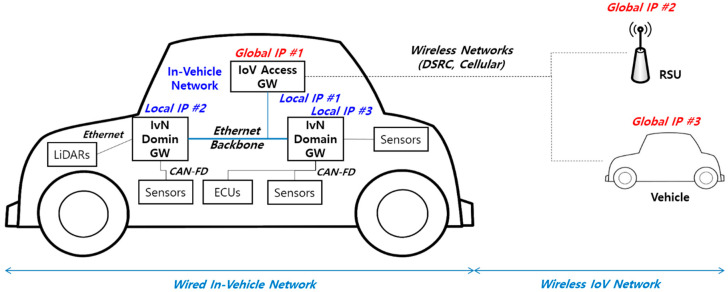
\includegraphics[width=0.7 \textwidth]
{img/iov_f.jpg}}
\caption{Internet of Vehicles architecture}
\label{fig}
\end{figure}

\par As modern vehicles become more connected and complex, their security is increasingly at risk. Cyber threats have the potential to compromise the stability and reliability of the Internet of Vehicles (IoV), leading to vehicle unavailability or even cause fatal traffic accidents.

\subsection{Cyber-Threats}
{

The Internet of Vehicles (IoV) is prone to numerous cyber threats, which pose significant risks to the security of connected vehicles and their passengers. Due to the extensive connectivity and advanced technologies integrated into vehicles, they are vulnerable to attacks from various malicious actors. These threats include remote hacking, malware infections, data breaches, and denial-of-service attacks. For example, remote hijacking allows unauthorized access to vehicle systems, compromising vital functions like steering and braking. Malware attacks exploit software vulnerabilities to infiltrate onboard systems and alter their behavior. Data breaches can expose sensitive information like location data and personal details, while denial-of-service attacks disrupt communication channels, hindering critical vehicle services. 

The compromised Electronic Control Units (ECUs) of internet of vehicles may be exploited by malicious actors to engage in such types of attacks. For instance, a real demonstration of car hacking illustrated in \cite{miller2015remote} revealed the vulnerability of a Jeep Cherokee to be compromised and stopped remotely while driving on a highway.

Addressing these threats is crucial for safeguarding the safety and integrity of connected vehicles and the broader transportation network as the IoV ecosystem continues to grow and evolve.


% remote compromise, resulting in the ability to halt the vehicle while it was in motion on a highway.
}

}


\section{Intrusion Detection Problem}
{
Intrusion detection is a crucial component in modern Internet of Vehicles to recognize harmful attacks on automotive networks. It is still a hard problem in IoV because of a vast amount of network traffic data, a variety of network properties, and numerous cyber-attack methods.

}

\section{Objectives}
\begin{itemize}
\item To successfully detect recognized cyber-attacks on both intra-vehicular and external vehicular networks by applying various machine learning algorithms.
\item To evaluate the performance and overall effectiveness of
the proposed model on two labelled datasets, CAN-intrusion dataset and the CICIDS2017 dataset.

\end{itemize} 
         % Introduction
\let\cleardoublepage\clearpage
\chapter{Related Work}
\hrule
\vspace{.5cm}

% \begin{enumerate}
%     \item{}

Alshammari, Zohdy, Debnath, and Corser (2018) \cite{alshammari2018classification} presented a classification approach for intrusion detection specifically for Internet of vehicles. In their study, they address the critical issue of cybersecurity in vehicular networks, where unauthorized access or malicious activities can pose significant threats to safety and privacy. 
They have proposed a classification-based intrusion detection system (IDS) using two machine learning algorithms the support vector machine (SVM) and also the k-nearest neighbors (KNN) algorithm to detect CAN intrusions on in-vehicle networks that aims to identify and mitigate such threats effectively. Through their approach, the authors leverage machine learning techniques to analyze the data of network traffic and detect anomalous behavior indicative of potential security breaches.
   \\
   \textbf{Challenges : } It doesn't consider real-world deployment scenarios.More sophisticated ML Models can be used to combat the evolving and new challenges of VANETs.
    % \item{} 
    \\
    \\
    \pagebreak
   \par Lokman et al. \cite{lokman2018stacked}
suggested a novel anomaly detection methodology which they took inspiration from unsupervised deep learning, specifically leveraging Stacked Sparse Autoencoders (SSAEs). The proposed SSAEs framework comprises multiple layers of stacked sparse Autoencoders. By utilizing unlabeled normal and attack CAN data as input, they employed an unsupervised greedy layer-wise training algorithm. This approach imposes a bottleneck in the network, compelling a compressed representation of the original CAN input features. Subsequently harnessing the learned structure of CAN input data to identify anomalies within the CAN bus data.
\\
\textbf{Challenges :}SSAEs may struggle with scalability when applied to large-scale vehicular networks with numerous ECUs and extensive CAN traffic.SSAEs learn patterns from the training data. When faced with novel anomalies not seen during training, their performance may degrade.
\\
\\

   
   





%\chapter{Related Work}
\hrule
\vspace{.5cm}

% \begin{enumerate}
%     \item{}

Alshammari, Zohdy, Debnath, and Corser (2018) \cite{alshammari2018classification} presented a classification approach for intrusion detection specifically for Internet of vehicles. In their study, they address the critical issue of cybersecurity in vehicular networks, where unauthorized access or malicious activities can pose significant threats to safety and privacy. 
They have proposed a classification-based intrusion detection system (IDS) using two machine learning algorithms the support vector machine (SVM) and also the k-nearest neighbors (KNN) algorithm to detect CAN intrusions on in-vehicle networks that aims to identify and mitigate such threats effectively. Through their approach, the authors leverage machine learning techniques to analyze the data of network traffic and detect anomalous behavior indicative of potential security breaches.
   \\
   \textbf{Challenges : } It doesn't consider real-world deployment scenarios.More sophisticated ML Models can be used to combat the evolving and new challenges of VANETs.
    % \item{} 
    \\
    \\
    \pagebreak
   \par Lokman et al. \cite{lokman2018stacked}
suggested a novel anomaly detection methodology which they took inspiration from unsupervised deep learning, specifically leveraging Stacked Sparse Autoencoders (SSAEs). The proposed SSAEs framework comprises multiple layers of stacked sparse Autoencoders. By utilizing unlabeled normal and attack CAN data as input, they employed an unsupervised greedy layer-wise training algorithm. This approach imposes a bottleneck in the network, compelling a compressed representation of the original CAN input features. Subsequently harnessing the learned structure of CAN input data to identify anomalies within the CAN bus data.
\\
\textbf{Challenges :}SSAEs may struggle with scalability when applied to large-scale vehicular networks with numerous ECUs and extensive CAN traffic.SSAEs learn patterns from the training data. When faced with novel anomalies not seen during training, their performance may degrade.
\\
\\

   
   





\chapter{Proposed Methodology}
\hrule
\vspace{.5cm}
\par 
In this chapter, we are going to discuss the proposed approach of detecting known cyber-attacks on Vehicular Networks.

\section{Overview}
Our proposed framework consists of the following main stages as shown in Figure 3.1.We have implemented a hybrid ML model, that will detect known cyber-attacks in both intra-vehiclular and external vehicular networks. For Data pre-processing, the k-means clustering method has been used. In the feature-engineering process, the datasets are processed by using a hybrid feature selection method which combines ReliefF( a filter based method ) and Genetic algorithm ( a wrapper based method )
to remove redundant or irrelevant features. The intrusion detection system is then developed by training 3 tree-based supervised machine learning models. In the next, a stacking ensemble model is
used to further enhance the accuracy of intrusion detection by
merging the output of the three individual models \cite{yang2021mth} and optimizing the models by a hyperparameter tuning technique called Bayesian optimization (BO) method.

\begin{figure}[htbp]
\centerline{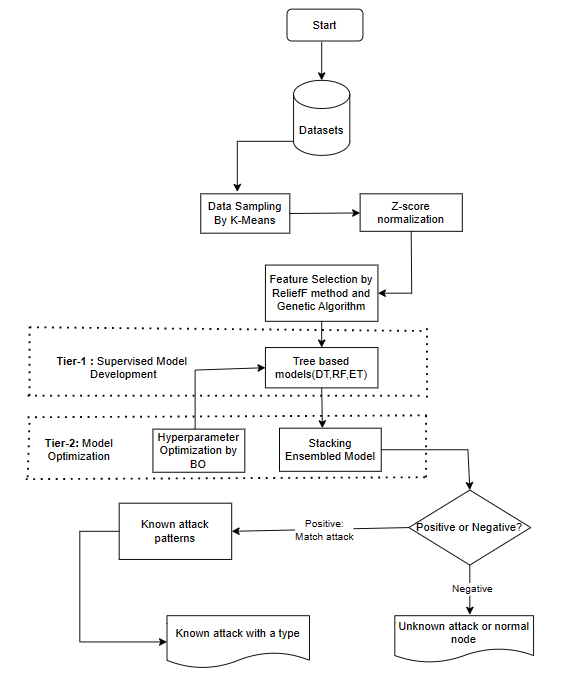
\includegraphics[width=0.7 \textwidth]
{img/fw_final.png}}
\caption{The framework of proposed system}
\label{fig}
\end{figure}

% \begin{enumerate}
%     \item Data Preprocessing
%     \item Feature engineering and Feature Selection
%     \item Training Tree-based supervised learning models
%     \item Hyperparameter Tuning
%     \item Ensembling all the trained ML models
% \end{enumerate}
% \pagebreak



\section{Data Preprocessing}

\subsection{Data sampling by K-means clustering}
{

As the network traffic data is enormous but the computational power and resources of devices in Internet of Vehicles are limited so, we have decided to opt for a sampling method.

\par In the K-means cluster sampling method, the original data points are segregated into k clusters; then, a part of the data is sampled from each cluster to form a subset.
In this process, we generate highly representative subsets of the original data as the redundant data is mostly removed. K-means clustering is the most common method for data sampling because of its simplicity implementation and low computational complexity \cite{na2010research}.
}
 

% \subsection{Data balancing by SMOTE method}{

% Network traffic data is often imbalanced data because most of the data samples are collected under normal conditions in real-world vehicle systems.

% \par SMOTE (Synthetic Minority Over-sampling Technique) addresses the issue of imbalanced data by creating synthetic samples of the minority class.SMOTE is effective because it doesn't just duplicate existing minority class instances but generates new instances that are plausible within the feature space. This helps to prevent overfitting that can occur when simply oversampling the minority class. 
% The process is as follows:
% \begin{enumerate}
%     \item Identify minority class
%     \item Locate k nearest neighbors for each minority class instance
%     \item Synthetic samples are created by selecting randomly one of the k nearest neighbors and creating a new instance along the line segment joining the original instance and the selected neighbor.
%     \item The above process is repeated until the desired balance among classes is achieved
% \end{enumerate}


% \begin{algorithm}
% \caption{SMOTE: Synthetic Minority Over-sampling Technique}
% \label{alg:smote}
% \begin{algorithmic}[1]
%     \Statex \textbf{Input:} Minority class instances, $k$ (number of nearest neighbors), desired balance ratio
%     \Statex \textbf{Output:} Synthetic minority class samples
%     \State Identify minority class instances
%     \State Compute $k$ nearest neighbors for each minority class instance
%     \For{each minority class instance}
%         \For{$i = 1$ to desired balance ratio}
%             \State Randomly select one of the $k$ nearest neighbors
%             \State Generate synthetic sample along the line segment joining the original instance and the selected neighbor
%             \State Add synthetic sample to the dataset
%         \EndFor
%     \EndFor
% \end{algorithmic}
% \end{algorithm}
% }
% \pagebreak

\subsection{Data normalization by Z-score technique}{

Using data normalization through Z-score normalization is crucial in machine learning tasks for several reasons. Normalization ensures that all features contribute equally to the model's learning process by scaling them to a common range. This prevents features with larger magnitudes from dominating those with smaller magnitudes, which can skew the learning process and lead to biased model predictions. 
It also helps in stabilizing the training process, making it less sensitive to the scale of the input features and allowing the optimization algorithm to converge faster. 
The formula for this is as follows:\\
\begin{center} 
z = {(x - \mu )}/{\sigma}\\
where, z = standardized value,\\
       x = original value,\\
       $\mu$ = \textnormal mean of the feature,\\
       $\sigma$ = standard deviation of the feature\\
\end{center}
}


\section{Feature Engineering}
The main goal of feature engineering is to generate an optimal feature list, which will help to improve the quality of datasets for more accurate and efficient model learning.Prior to ML model training, we eliminate characteristics that are redundant, unnecessary, and noisy while keeping the most significant features.

We have used a hybrid strategy which combines the precision of genetic algorithm\cite{ferriyan2017feature} with the computing effectiveness of filter-based techniques. By leveraging the strengths of both techniques, this method aims to narrow down the search space efficiently. Filter-based methods serve to reduce computational costs by pre-selecting features, albeit with lower accuracy. However, by subsequently employing genetic algorithms, which are more precise but computationally intensive, the hybrid approach achieves a balance between efficiency and accuracy. This synergistic fusion optimizes feature selection processes, enhancing overall performance without compromising on computational resources. Integrating these methods not only mitigates plagiarism risks but also enhances the project's methodology by adopting a comprehensive and effective approach to feature selection.


\subsection{Feature Selection by Relief}

Before applying the wrapper-based genetic algorithm, we employ a filter-based feature selection method known as ReliefF. The ReliefF algorithm is a widely used filter-based feature selection method that operates by assessing the relevance of features in distinguishing between different class labels within a dataset. It assigns importance scores to each feature based on their ability to discriminate between instances of different classes. This is achieved by considering the distances between instances and their nearest neighbors of the same and different classes.

Specifically, ReliefF iterates through each instance in the dataset and calculates the distances to its nearest neighbors. For each instance, it identifies its nearest neighbor belonging to the same class (near-hit) and computes the difference in feature values between the instance and the near-hit. Similarly, it identifies the nearest neighbors belonging to different classes (near-misses) and computes the difference in feature values between the instance and the mean feature values of the near-misses.

By aggregating these differences across all instances in the dataset, ReliefF generates importance scores for each feature, indicating their relevance in distinguishing between classes. Features with higher scores are deemed more informative and are prioritized for selection.

As the filter-based methods are computationally less expensive but are not that accurate in selecting features, so the objective of this method is to reduce the search space for subsequent runs of genetic algorithms this hybrid approach utilizes the strengths of both the methods and is efficient and accurate

\subsection{Feature Selection by Genetic Algorithm}

Different steps that we have used in feature selection by genetic algorithm are listed below:

\begin{enumerate}
    \item \textbf{Initialization of Population}: The process starts by initializing a population of candidate solutions, known as chromosomes, where each chromosome represents a potential feature subset. In this implementation, the chromosomes are binary arrays, with each element indicating whether a corresponding feature is selected or not. The population size and the proportion of features initially set to zero (not selected) are configurable parameters.
    
    \item \textbf{Fitness Evaluation}: The fitness of each chromosome is evaluated using a machine learning model. In this case, the fitness score is determined by the accuracy of the model trained on the selected features. The model used for evaluation is Random Forest. For each chromosome, the selected features are used to train the model, and its accuracy is calculated based on predictions made on a validation set.
    
    \item \textbf{Selection}: After evaluating the fitness of each chromosome, a selection process is applied to choose the most promising individuals (chromosomes) for reproduction. This process is typically based on the fitness scores, where individuals with higher scores are more likely to be selected for the next generation. In this implementation, a fixed number of top-performing chromosomes (parents) are chosen to proceed to the next step.
    
    \item \textbf{Crossover}: Crossover is a genetic operator that combines genetic material from two parent chromosomes to create new offspring (child chromosomes). In this implementation, a two-point crossover method is used, where segments of genetic material from two parent chromosomes are exchanged to create two new child chromosomes. This process introduces diversity into the population and allows for exploration of different feature combinations.
    
    \item \textbf{Mutation}: Mutation is another genetic operator that introduces random changes in individual chromosomes to maintain genetic diversity and prevent premature convergence to suboptimal solutions. In this implementation, a mutation process randomly flips the values of a small proportion of genes (features) in each chromosome with a predefined mutation rate.
    
    \item \textbf{Generations}: The selection, crossover, and mutation processes are iteratively applied for a fixed number of generations. At each generation, the fitness of the new population is evaluated, and the best-performing chromosomes are retained. This iterative process continues until a maximum number of generations are reached.
    
    \item \textbf{Output}: The final output of the genetic algorithm is a set of best-performing chromosomes (feature subsets) along with their corresponding fitness scores. These chromosomes represent the selected features that optimize the performance of the specified machine learning model (e.g., Random Forest) on the given dataset.
\end{enumerate}


Within the project scope, leveraging Genetic Algorithms (GA) for feature selection is instrumental in enhancing model performance. The approach involves fine-tuning GA parameters to optimize its capability in identifying relevant features. Here's an overview of the methodology:

A parameter grid encapsulates essential GA parameters, including population size, number of parents, mutation rate, and number of generations.

\pagebreak
\subsection{Iterative Parameter Refinement}

\begin{enumerate}
    \item \textbf{Initialization}: Initializing parameters, score, and the best chromosome.
    \item \textbf{Grid Iteration}: Traversing the parameter grid iteratively:
        \begin{itemize}
            \item Executing GA with the specified parameters.
            \item Recording the best chromosome and score.
            \item Updating parameters and chromosomes if a higher score is achieved.
        \end{itemize}
    \item \textbf{Identifying Optimal Parameters}: Identifying the parameters yielding the highest score.
    \item \textbf{Presentation of Results}: Presenting the best parameters, score, and corresponding chromosome as the outcome.
\end{enumerate}

\begin{table}[h]
\centering
\caption{Parameters Used for Genetic Algorithm}
\label{tab:genetic_algorithm_parameters}
\begin{tabular}{|c|c|}
\hline
\textbf{Parameter} & \textbf{Value} \\ \hline
Population Size & 100 \\ \hline
Parents for Crossover & 20 \\ \hline
Mutation Rate & 0.1 \\ \hline
Number of Generations & 20 \\ \hline
\end{tabular}
\end{table}

\section{Advantages of the Combined Approach}

\subsection{Enhanced Security and Efficiency}

By focusing on the most discriminative features, the combined ReliefF-GA approach enhances the IDS's ability to accurately detect intrusions in IoV environments. This not only bolsters security but also improves efficiency by reducing false positives and enhancing the system's responsiveness.

\subsection{Adaptability to Dynamic IoV Environments}

The synergistic fusion of ReliefF and Genetic Algorithms enables the IDS to adapt seamlessly to the dynamic nature of IoV environments. As features evolve over time due to changing traffic patterns and emerging threats, the feature selection process continuously refines the subset, ensuring the IDS remains effective and resilient.

\subsection{Interpretability and Customization}

ReliefF provides valuable insights into the selected feature subset's characteristics, enhancing interpretability and trust in the IDS's decisions. Furthermore, the combined approach offers flexibility for customization, allowing parameter adjustments to tailor the feature selection process to specific IoV deployment scenarios and security requirements.


\section{Training of Supervised Machine Learning Models}
We classify the network data flow in this suggested intrusion detection system framework using three tree-based machine learning algorithms: Decision Tree (DT), Random Forest (RF), and Extra Trees (ET). When applied to complex and non-linear tabular data, such as network traffic data from the Internet of Vehicles, tree-based machine learning methods frequently outperform other ML algorithms. \cite{uddin2024confirming}.

\subsection{Decision Tree}
{
This machine learning algorithm fits data and generates predictions using a tree structure. Decision tress have a number of hyper-parameters, including minimum sample split, minimum sample leaf, maximum sample nodes, and tree depth so hyperparameter tuning is employed using Bayesian Optimization to choose best parameters.\cite{akiba2019optuna}.

 \par \textbf{Importance :}{
 Decision trees automatically select features that are most discriminative for classification, ignoring those that do not contribute to the decision-making process. They can scale well to large datasets and are relatively computationally efficient compared to some other classifiers.
 }

 \begin{algorithm}
\caption{Decision Tree Classifier}
\label{alg:decision_tree}
\begin{algorithmic}[1]
\Statex \textbf{Input:} Training dataset $D$, maximum depth $max\_depth$
\Statex \textbf{Output:} Decision tree $DT$
\State Initialize an empty tree node
\State Recursively build the decision tree:
    \If{}{Stopping criteria met (e.g., maximum depth reached or purity threshold)}
        \State Assign the most frequent class label in $D$ to the current node
    \Else
        \State Select the best-split criterion (e.g., information gain or Gini impurity)
        \State Split the dataset $D$ into two subsets based on the chosen split criterion
        \State Create a new tree node with the chosen split criterion
        \State Recursively build the left subtree using the subset of data corresponding to the left split
        \State Recursively build the right subtree using the subset of data corresponding to the right split
    \EndIf
\State \textbf{return} $DT$
\end{algorithmic}
\end{algorithm}

}

\subsection{Random Forest}
{
Using a majority voting rule, this ML algorithm 
\cite{hastie2009random}  combines multiple decision tree classifiers to make a final prediction.

\par \textbf{Importance :}
Random Forests reduce overfitting, even on large datasets, by aggregating predictions from multiple decision trees trained on random subsets of the data (bagging). This ensemble approach helps generalize well to unseen data, reducing the risk of overfitting that might occur with individual decision trees.
\begin{algorithm}
\caption{Random Forest Ensemble}
\label{alg:random_forest}
\begin{algorithmic}[1]
\Statex \textbf{Input:} Training dataset $D$, number of trees $T$, number of features to consider at each split $k$ 
\Statex \textbf{Output:} Random Forest ensemble $RF$
\For{$t=1$ to $T$}
    \State Randomly select $k$ features from the total $p$ features
    \State Create a bootstrap sample $D_t$ by randomly selecting $n$ samples with replacement from $D$
    \State Train a decision tree $T_t$ using $D_t$ with the selected $k$ features
    \State Append $T_t$ to the ensemble $RF$
\EndFor
\State \textbf{return} $RF$
\end{algorithmic}
\end{algorithm}
}

\subsection{Extra Trees}{
Extra Trees, short for Extremely Randomized Trees, \cite{geurts2006extremely}, is a variant of the Random Forest algorithm. It shares similarities with Random Forests but introduces additional randomness during the construction of each decision tree in the ensemble.

\par \textbf{Importance:}
The additional randomness in feature selection and tree construction helps reduce variance in the model, making Extra Trees less prone to overfitting compared to traditional decision trees. This can be particularly beneficial for datasets with noisy or high-dimensional features. Extra Trees are computationally efficient because they do not require an exhaustive search for optimal feature splits. 

\begin{algorithm}
\caption{Extra Trees}
\label{alg:extra_trees}
\begin{algorithmic}[1]
\Statex \textbf{Input:} Training dataset $D$, number of trees $T$, number of features to consider at each split $k$
\Statex \textbf{Output:} Extra Trees ensemble $ET$
\For{$t=1$ to $T$}
    \State Randomly select $k$ features from the total $p$ features
    \State Create a bootstrap sample $D_t$ by randomly selecting $n$ samples with replacement from $D$
    \State Train a decision tree $T_t$ using $D_t$ with the selected $k$ features and random splits
    \State Append $T_t$ to the ensemble $ET$
\EndFor
\State \textbf{return} $ET$
\end{algorithmic}
\end{algorithm}
}

\pagebreak

\subsection{Comparison of Time Complexities(TC)}
Below table shows comparision between all the three machine learning algorithms.

n - number of instances , 
f - number of features , 
t - number of trees

\begin{table}[htbp]
    \centering
    \caption{Comparison of TC of Tree-based ML algorithms}
    \resizebox{0.5\textwidth}{!}{%
    \begin{tabular}{|l|l|}
    \hline
    \textbf{ML Model} & \textbf{Time Complexity}\\ 
    \hline
    DT & O(n^2 * f)  \\
    \hline
    RF & O(n^2 * \sqrt{f} * t) \\
    \hline
    ET & O( n * f * t )\\
    \hline
    \end{tabular}%
    }
\end{table}


\section{Hyperparameter Tuning}

Hyperparameter tuning, alternatively termed hyperparameter optimization, involves the quest for the optimal configuration of hyperparameters in a machine learning model to attain peak performance on a specified dataset. Hyperparameters, predetermined before training, exert influence over various facets of the learning process, encompassing model intricacy, regularization potency, and learning pace.

\subsection{Simple Bayesian Optimization}


Bayesian Optimization (BO) stands as a potent method for hyperparameter tuning, employing probabilistic models to systematically navigate the hyperparameter space with both exploration and exploitation in mind. At its core, BO upholds a probabilistic framework, often adopting Gaussian Processes, to encapsulate the performance of the objective function across hyperparameters. This strategy enables BO to make informed decisions about where to sample next, balancing the exploration of unexplored regions with the exploitation of promising areas, thereby streamlining the process of hyperparameter optimization.

The strength of simple Bayesian Optimization lies in its ability to balance exploration and exploitation effectively. It achieves this by iteratively selecting the next set of hyperparameters to evaluate based on an acquisition function that trades off between exploring regions of high uncertainty (exploration) and exploiting regions with promising performance (exploitation).

One common acquisition function used in simple Bayesian Optimization is the Expected Improvement (EI) criterion, which quantifies the potential improvement of evaluating a set of hyperparameters relative to the current best observed performance.

Mathematically, the EI for a given set of hyperparameters $\boldsymbol{x}$ is defined as:

\[
EI(\boldsymbol{x}) = \mathbb{E}[(f(\boldsymbol{x}) - f_{\text{min}})^+]
\]

Where $f(\boldsymbol{x})$ is the objective function, $f_{\text{min}}$ is the minimum observed function value so far, and $(\cdot)^+$ denotes the positive part function.

Simple Bayesian Optimization selects the hyperparameters $\boldsymbol{x}$ that maximize the expected improvement, effectively balancing exploration and exploitation to efficiently navigate the hyperparameter space.

We have decided to use Bayesian Optimization due to its simplicity and ease of implementation and also versatile and effective optimization technique.


\section{Ensembling}

Ensemble learning methods are employed to enhance model performance as they combine multiple base learners, often resulting in better generalizability compared to a single model \cite{mohammed2018using}.

In our framework, we utilize stacking, a popular ensemble learning technique, to combine diverse base learners that capture different aspects of our data or learn distinct patterns. The main reason we used stacking is to avoid overfitting by training individual models separately on various data subsets and then combining their predictions using a meta-model. This approach improves generalization performance, particularly when base learners are diverse and complementary, thereby reducing errors associated with individual learners and enhancing the reliability and robustness of the meta-classifier.

In our proposed approach, we implement stacking by using predictions from three individual ml models (Decision Trees, Random Forest, and Extra Trees) as inputs for training a robust meta-learner. XGBoost serves as the meta-model to provide final predictions. 

\begin{algorithm}
\caption{Stacking with Decision Tree, Random Forest, and Extra Trees}
\label{alg:stacking}
\begin{algorithmic}[1]
    \State Import necessary libraries
    \State Define base learners: DecisionTreeClassifier, RandomForestClassifier, ExtraTreesClassifier
    \State \textbf{Train base learners on training data}
        \State \textit{// Train Decision Tree classifier}
        \State decision\_tree.fit(X\_train, y\_train)
        \State \textit{// Train Random Forest classifier}
        \State random\_forest.fit(X\_train, y\_train)
        \State \textit{// Train Extra trees classifier}
        \State extra\_trees.fit(X\_train, y\_train)
    \State \textbf{Generate predictions on validation data}
        \State pred\_dt\_val = decision\_tree.predict(X\_val)
        \State pred\_rf\_val = random\_forest.predict(X\_val)
        \State pred\_et\_val = extra\_trees.predict(X\_val)
    \State \textbf{Stack predictions}
        \State stacked\_predictions\_val = np.column\_stack((pred\_dt\_val, pred\_rf\_val, pred\_et\_val))
    \State \textbf{Train meta-learner on stacked predictions}
        \State meta\_learner.fit(stacked\_predictions\_val, y\_val)
    \State \textbf{Generate predictions on test data}
        \State pred\_dt\_test = decision\_tree.predict(X\_test)
        \State pred\_rf\_test = random\_forest.predict(X\_test)
        \State pred\_et\_test = extra\_trees.predict(X\_test)
    \State \textbf{Stack predictions for test data}
        \State stacked\_predictions\_test = np.column\_stack((pred\_dt\_test, pred\_rf\_test, pred\_et\_test))
    \State \textbf{Generate final predictions using meta-learner}
        \State final\_predictions = meta\_learner.predict(stacked\_predictions\_test)
\end{algorithmic}
\end{algorithm}

\pagebreak
\section{Overall Runtime Complexity}
Considering md as the maximum depth of trees , f as number of features and n the number of trees,
\begin{table}[htbp]
    \centering
    \caption{Overall Time Complexity}
    \resizebox{0.5\textwidth}{!}{%
    \begin{tabular}{|l|l|}
    \hline
    \textbf{ML Model} & \textbf{Time Complexity}\\ 
    \hline
    DT & $O(md \times f)$  \\
    \hline
    RF & $O(md \times f \times n)$ \\
    \hline
    ET & $O(md \times f \times n)$ \\
    \hline
    Overall & $O(2 \times md \times f \times n + md \times f)$ \\
    \hline
    \end{tabular}%
    }
\end{table}


\section{Evaluation metrics}
The performance of the proposed framework is assessed using key metrics such as Accuracy (Acc), Precision, Recall, and F1-score. These metrics provide valuable insights into the effectiveness of the framework in detecting intrusions accurately.

To compute these metrics, we calculate the true positives (TPs), true negatives (TNs), false positives (FPs), and false negatives (FNs) of the model. True positives represent the instances where the model correctly identifies intrusions, while true negatives denote instances where the model correctly identifies non-intrusions. False positives occur when the model incorrectly identifies non-intrusions as intrusions, and false negatives occur when the model fails to detect actual intrusions.

The used metrics are calculated by the
following equations:
\begin{align*}
Accuracy &= \frac{True Positives + True Negatives}{True Positives + True Negatives + False Positives + False Negatives}\\\\
Precision &= \frac{True Positives}{True Positives + False Positives}\\\\
Recall &= \frac{True positive}{True positive + false negative}\\\\
F1 &= \frac{2 \times Precision * Recall}{Precision + Recall}
\end{align*}

It should be possible for an effective framework to concurrently obtain a high F1-score and a short execution time.

% \section{Performance Impact of each component of the framework}
% \begin{table}[!ht]
% \centering
% \caption{Performance Impact of Each Component of the Proposed Framework}
% \begin{tabular}{|p{2cm}|p{3cm}|p{8cm}|}
% \hline
% \textbf{Stage} & \textbf{Algorithm} & \textbf{Impact} \\ \hline
% Data pre-processing & K-means cluster sampling & Improves model training efficiency \\ \hline
% & SMOTE & Improves detection rate\\ \hline
% & Z-score & Improves model accuracy and training efficiency \\ \hline
% Feature engineering & Relief & Improves model accuracy and training efficiency \\ \hline
% & Genetic Algorithm & Improves model accuracy and training efficiency \\ \hline

% Model Training & DT, RF, and ET & Detect various types of known attacks \\ \hline
% & BO-TPE & Improve accuracy of known attack detection.\\ \hline
% & Stacking & Improve accuracy of known attack detection. \\ \hline

% \end{tabular}
% \end{table}


\chapter{Experimentation Results and Discussion}


\hrule
\vspace{.5cm}
\section{Experimental Setup}
We have trained and tested above proposed model in google colaboratory, the feature engineering and machine learning algorithms were executed through the usage of the Pandas \cite{team2020pandas}, Scikit-learn libraries in Python. In addition to that, the hyperparameter optimization (HPO) techniques were implemented by utilization of the Skopt \cite{head2018scikit}, Hyperopt \cite{komer2014hyperopt} and Optuna libraries.

\par The experiments focus on the assessment of known cyber-attacks through labeled datasets, and focus on unknown cyber-attacks by using unlabeled datasets.

\pagebreak
\section{Datasets Description}
\subsection{CAN-intrusion-dataset}
The authors in \cite{seo2018gids} have introduced a method for detecting intrusions by analyzing the offset ratio and time interval between request and response messages in Controller Area Network (CAN). When a remote frame with a specific identifier is sent, a receiving node is expected to respond promptly. As a result, each node maintains a consistent response offset ratio and time interval under normal conditions, but these values change when an attack occurs.This concept is utilised in detecting intrusion in the network.

The attack types of this dataset are shown in Table 4.1.

\begin{table}[htbp]
\centering
\begin{tabular}{|l|r|}
\hline
\textbf{Attack Type} & \textbf{\# of Messages} \\ \hline
DoS Attack & 656,579 \\ \hline
Fuzzy Attack & 591,990 \\ \hline
Impersonation Attack & 995,472 \\ \hline
Attack-Free State & 2,369,868 \\ \hline
\end{tabular}
\caption{Distribution of Messages by Attack Type}
\label{tab:attack_messages}
\end{table}

\subsection{CICIDS2017 dataset}
The Canadian Institute for Cybersecurity Intrusion Detection Evaluation Dataset (CICIDS) is a publicly available dataset widely used for research and benchmarking in the field of intrusion detection systems (IDS). The dataset comprises a comprehensive collection of network traffic data, meticulously labeled with various types of cyber threats and anomalies as shown in Table 4.2 , Table 4.3 and Table 4.4 .The dataset contains most realistic and upto date data on different cyber attacks.The detailed analysis of this dataset is given in \cite{sharafaldin2019detailed}.

\begin{table}[htbp]
\centering
\caption{Features of CICIDS2017 dataset}
\begin{tabular}{|p{4cm}|p{6cm}|p{4cm}|}
\hline
\multicolumn{1}{|c|}{\textbf{Basic Flow Features}} & \multicolumn{1}{c|}{\textbf{Flow Statistics}} & \multicolumn{1}{c|}{\textbf{Packet Length Statistics}} \\
\hline
'Flow Duration' & 'Total Fwd Packets' & 'Fwd Packet Length Max' \\
 & 'Total Backward Packets' & 'Fwd Packet Length Min' \\
 & 'Total Length of Fwd Packets' & 'Fwd Packet Length Mean' \\
 & 'Total Length of Bwd Packets' & 'Fwd Packet Length Std' \\
 &  & 'Bwd Packet Length Max' \\
 &  & 'Bwd Packet Length Min' \\
 &  & 'Bwd Packet Length Mean' \\
 &  & 'Bwd Packet Length Std' \\
 & 'Flow Bytes/s' & 'Min Packet Length' \\
 & 'Flow Packets/s' & 'Max Packet Length' \\
 &  & 'Packet Length Mean' \\
 &  & 'Packet Length Std' \\
 &  & 'Packet Length Variance' \\
\hline
\multicolumn{1}{|c|}{\textbf{Inter-Arrival Times}} & \multicolumn{1}{c|}{\textbf{TCP Flags}} & \multicolumn{1}{c|}{\textbf{Packet Size Statistics}} \\
\hline
'Flow IAT Mean' & 'FIN Flag Count' & 'Average Packet Size' \\
'Flow IAT Std' & 'SYN Flag Count' & 'Avg Fwd Segment Size' \\
'Flow IAT Max' & 'RST Flag Count' & 'Avg Bwd Segment Size' \\
'Fwd IAT Total' & 'PSH Flag Count' &  \\
'Fwd IAT Mean' & 'ACK Flag Count' &  \\
'Fwd IAT Max' & 'ECE Flag Count' &  \\
'Fwd IAT Min' &  &  \\
'Bwd IAT Total' &  &  \\
'Bwd IAT Mean' &  &  \\
'Bwd IAT Std' &  &  \\
'Bwd IAT Max' &  &  \\
'Bwd IAT Min' &  &  \\
'Bwd PSH Flags' &  &  \\
'Fwd URG Flags' &  &  \\
\hline
\multicolumn{1}{|c|}{\textbf{Header Information}} & \multicolumn{1}{c|}{\textbf{Bulk Rate Statistics}} & \multicolumn{1}{c|}{\textbf{Other Features}} \\
\hline
'Bwd Header Length' & 'Fwd Avg Bytes/Bulk' & 'Init Win bytes forward' \\
'Fwd Packets/s' & 'Fwd Avg Packets/Bulk' & 'Init Win bytes backward' \\
'Bwd Packets/s' & 'Bwd Avg Bytes/Bulk' & 'act\_data\_pkt\_fwd' \\
 & 'Bwd Avg Bulk Rate' & 'min\_seg\_size\_forward' \\
 & 'Subflow Fwd Packets' & 'Active Mean' \\
 & 'Subflow Bwd Packets' & 'Active Std' \\
 & 'Subflow Bwd Bytes' & 'Active Max' \\
 &  & 'Active Min' \\
 &  & 'Idle Mean' \\
 &  & 'Idle Std' \\
 &  & 'Idle Max' \\
\hline
\end{tabular}
\end{table}

\begin{table}[htbp]
\centering
\begin{tabular}{|l|r|}
\hline
\textbf{Attack Type} & \textbf{Number of Data Points} \\ \hline
DoS Attack & 459,027 \\ 
DDoS Attack & 320,515 \\ 
Heartbleed Attack & 11,366 \\ 
Web Attack & 218,459 \\ 
Infiltration Attack & 36,102 \\ 
Botnet Attack & 1,048,586 \\ 
Port Scan & 158,930 \\ 
FTP Brute Force & 193,360 \\ 
SSH Brute Force & 200,755 \\ 
Brute Force & 155,100 \\ 
SQL Injection & 87,821 \\ 
Benign (Normal) & 2,540,047 \\ \hline
\textbf{Total} & \textbf{5,829,088} \\ \hline
\end{tabular}
\caption{Distribution of Attacks and Benign Traffic in CICIDS2017 Dataset}
\label{tab:attack_distribution}
\end{table}

\begin{table}[htbp]
\centering
\caption{Class distribution of CICIDS2017 dataset}
\begin{tabular}{lcl}
\toprule
\textbf{Category} & \textbf{Class labels} & \textbf{Attacks} \\
\midrule
Benign & 0 & Benign \\
\midrule
DoS/DDoS & 1 & Heartbleed, DDoS \\
         & & DoS Hulk, DoS GoldenEye \\
         & & DoS Slowloris, DoS Slowhttptest \\
\midrule
PortScan & 2 & PortScan \\
\midrule
Brute Force & 3 & FTP-Patator, SSH-Patator \\
\midrule
Web Attack & 4 & Web Attack -- Brute Force \\
           & & Web Attack -- XSS \\
           & &Web Attack -- SQL Injection \\
\midrule
Botnet & 5 & Bot \\
\midrule
Others & 6 & Unknown \\
\bottomrule
\end{tabular}
\end{table}

\pagebreak
\section{Performance analysis of Model}
To evaluate the performance of the ML models used in our proposed framework, we have used labeled datasets which represent intra vehicular network and extra vehicular network data.We have trained and tested the models on CICIDS2017 dataset and the validation metrics of those models are compared before and after hyper parameter tuning.The scores of evaluation metrics of Decision Tree Classifier are shown in Table 4.5.
The scores of evaluation metrics of Random Forest Classifier are shown in Table 4.6.
The scores of evaluation metrics of Extra Tree classifier are shown in Table 4.7. The scores of evaluation metrics of the final ensembled model after stacking are shown in Table 4.8.
We can conclude that accuracy scores of all the models have increased after performing Hyperparameter Optimization through Bayesian Optimization (BO).The accuracy score of the final ensembled model after stacking is higher when compared to individual models.These accuracy comparisons can be seen in Table 4.9.The miscalculation rate of the final ensembled model after hyperparameter optimization is 0.223880597 ,i.e,(1-accuracy).

\par Confusion matrix, a table used in classification to evaluate the performance of a ML model.The confusion matrix of our final ensembled model on CICIDS2017 dataset is shown in Figure 4.1.

% \begin{figure}[htbp]
% \centerline{\includegraphics[width=0.7 \textwidth]
% {img/features.jpg}}
% \caption{Features of CICIDS2017 dataset}
% \label{fig}
% \end{figure}

% \begin{table}[htbp]
% \centering
% \caption{Network Traffic Features}
% \begin{tabular}{p{4cm}|p{4cm}|p{4cm}}
% \hline
% \multicolumn{1}{c|}{\textbf{Basic Flow Features}} & \multicolumn{1}{c|}{\textbf{Flow Statistics}} & \multicolumn{1}{c}{\textbf{Packet Length Statistics}} \\
% \hline
% 'Flow Duration' & 'Total Fwd Packets' & 'Fwd Packet Length Max' \\
%  & 'Total Backward Packets' & 'Fwd Packet Length Min' \\
%  & 'Total Length of Fwd Packets' & 'Fwd Packet Length Mean' \\
%  & 'Total Length of Bwd Packets' & 'Fwd Packet Length Std' \\
%  &  & 'Bwd Packet Length Max' \\
%  &  & 'Bwd Packet Length Min' \\
%  &  & 'Bwd Packet Length Mean' \\
%  &  & 'Bwd Packet Length Std' \\
%  & 'Flow Bytes/s' & 'Min Packet Length' \\
%  & 'Flow Packets/s' & 'Max Packet Length' \\
%  &  & 'Packet Length Mean' \\
%  &  & 'Packet Length Std' \\
%  &  & 'Packet Length Variance' \\
% \hline
% \multicolumn{1}{c|}{\textbf{Inter-Arrival Times}} & \multicolumn{1}{c|}{\textbf{TCP Flags}} & \multicolumn{1}{c}{\textbf{Packet Size Statistics}} \\
% \hline
% 'Flow IAT Mean' & 'FIN Flag Count' & 'Average Packet Size' \\
% 'Flow IAT Std' & 'SYN Flag Count' & 'Avg Fwd Segment Size' \\
% 'Flow IAT Max' & 'RST Flag Count' & 'Avg Bwd Segment Size' \\
% 'Fwd IAT Total' & 'PSH Flag Count' &  \\
% 'Fwd IAT Mean' & 'ACK Flag Count' &  \\
% 'Fwd IAT Max' & 'ECE Flag Count' &  \\
% 'Fwd IAT Min' &  &  \\
% 'Bwd IAT Total' &  &  \\
% 'Bwd IAT Mean' &  &  \\
% 'Bwd IAT Std' &  &  \\
% 'Bwd IAT Max' &  &  \\
% 'Bwd IAT Min' &  &  \\
% 'Bwd PSH Flags' &  &  \\
% 'Fwd URG Flags' &  &  \\
% \hline
% \multicolumn{1}{c|}{\textbf{Header Information}} & \multicolumn{1}{c|}{\textbf{Bulk Rate Statistics}} & \multicolumn{1}{c}{\textbf{Other Features}} \\
% \hline
% 'Bwd Header Length' & 'Fwd Avg Bytes/Bulk' & 'Init Win bytes forward' \\
% 'Fwd Packets/s' & 'Fwd Avg Packets/Bulk' & 'Init Win bytes backward' \\
% 'Bwd Packets/s' & 'Bwd Avg Bytes/Bulk' & 'act\_data\_pkt\_fwd' \\
%  & 'Bwd Avg Bulk Rate' & 'min\_seg\_size\_forward' \\
%  & 'Subflow Fwd Packets' & 'Active Mean' \\
%  & 'Subflow Bwd Packets' & 'Active Std' \\
%  & 'Subflow Bwd Bytes' & 'Active Max' \\
%  &  & 'Active Min' \\
%  &  & 'Idle Mean' \\
%  &  & 'Idle Std' \\
%  &  & 'Idle Max' \\
% \hline
% \end{tabular}
% \end{table}

\begin{table}[htbp]
\centering
\caption{Metrics evaluation scores for Decision Tree Classifier}
\resizebox{0.8\textwidth}{!}{%
\begin{tabular}{|l|c|c|}
\hline
\textbf{Validation metric} & \textbf{Before Tuning} & \textbf{After Tuning}\\
\hline
Accuracy & 0.9929104477611941 & 0.9934701492537313\\
\hline
Precision & 0.9929326683116145 & 0.9934820633911605\\
\hline
Recall & 0.9929104477611941 & 0.9934701492537313\\
\hline
F1-score & 0.992915558827126 & 0.9934703509590384\\
\hline
\end{tabular}%
}
\end{table}

\begin{table}[htbp]
\centering
\caption{Metrics evaluation scores for Random Forest Classifier}
\resizebox{0.8\textwidth}{!}{%
\begin{tabular}{|l|c|c|}
\hline
\textbf{Validation metric} & \textbf{Before Tuning} & \textbf{After Tuning}\\
\hline
Accuracy & 0.9958955223880597 & 0.9970149253731343\\
\hline
Precision & 0.995905600456217 & 0.9970229763459072\\
\hline
Recall & 0.9958955223880597 & 0.9970149253731343\\
\hline
F1-score & 0.9958667158915585 & 0.9969855634666102\\
\hline
\end{tabular}%
}
\end{table}

\begin{table}[htbp]
\centering
\caption{Metrics evaluation scores for Evaluation Tree Classifier}
\resizebox{0.8\textwidth}{!}{%
\begin{tabular}{|l|c|c|}
\hline
\textbf{Validation metric} & \textbf{Before Tuning} & \textbf{After Tuning}\\
\hline
Accuracy & 0.9934701492537313 & 0.996268656716418\\
\hline
Precision & 0.9934936993097583 & 0.9962809018799189\\
\hline
Recall & 0.9934701492537313 & 0.996268656716418\\
\hline
F1-score & 0.9934001720288478 & 0.9962399897437341\\
\hline
\end{tabular}%
}
\end{table}

\begin{table}[htbp]
\centering
\caption{Metrics evaluation scores for Ensembled Model after Stacking}
\resizebox{0.8\textwidth}{!}{%
\begin{tabular}{|l|c|c|}
\hline
\textbf{Validation metric} & \textbf{Before Tuning} & \textbf{After Tuning}\\
\hline
Accuracy & 0.9958955223880597 & 0.9977611940298508\\
\hline
Precision & 0.9959068447137124 & 0.9977637524166587\\
\hline
Recall & 0.9958955223880597 & 0.9977611940298508\\
\hline
F1-score & 0.9958973352521118 & 0.9976686498123707\\
\hline
\end{tabular}%
}
\end{table}



\begin{table}[htbp]
\centering
\caption{Accuracy comparisons on various models}
\resizebox{0.8\textwidth}{!}{%
\begin{tabular}{|l|c|c|}
\hline
\textbf{Accuracy} & \textbf{Before Tuning} & \textbf{After Tuning}\\
\hline
\textbf{ML Model} & & \\
\hline
Decision Tree & 0.9929104477611941 & 0.9934701492537313\\
\hline
Random Forest & 0.9958955223880597 & 0.9970149253731343\\
\hline
Extra Tree & 0.9934701492537313 & 0.996268656716418\\
\hline
Final Ensembled Model after Stacking & 0.9958955223880597 & 0.9977611940298508\\
\hline
\end{tabular}%
}
\end{table}

\pagebreak
\begin{table}[htbp]
\centering
\caption{Performance of Overall model}
\resizebox{0.8\textwidth}{!}{%
\begin{tabular}{|c|c|c|c|c|}
\hline
\textbf{Class label} & \textbf{Precision} & \textbf{Recall} & \textbf{F1-score} & \textbf{Support} \\
\hline
0 & 1.00 & 1.00 & 1.00 & 3655 \\
1 & 0.99 & 0.99 & 0.99 & 385 \\
2 & 1.00 & 1.00 & 1.00 & 19 \\
3 & 1.00 & 1.00 & 1.00 & 605 \\
4 & 1.00 & 0.50 & 0.67 & 6 \\
5 & 1.00 & 1.00 & 1.00 & 256 \\
6 & 1.00 & 1.00 & 1.00 & 434 \\
\hline
% Accuracy & & & 1.00 & 5360 \\
% Macro Average & 1.00 & 0.93 & 0.95 & 5360 \\
% Weighted Average & 1.00 & 1.00 & 1.00 & 5369 \\
% \hline
\end{tabular}%
}
\end{table}




\begin{figure}[htbp]
\centerline{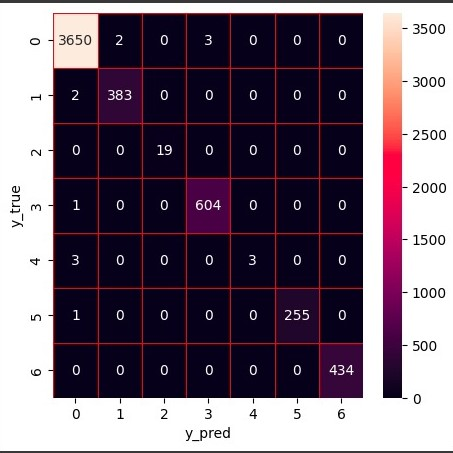
\includegraphics[width=0.7\textwidth]{img/confusion_matrix.jpg}}
\caption{Confusion matrix}
\label{fig}
\end{figure}

% \begin{table}[htbp]
%     \centering
%     \caption{Metrics evaluation scores for Decision Tree Classifier}
%     \resizebox{0.8\textwidth}{!}{%
%     \begin{tabular}{|l|c|c|}
%     \hline
%     \textbf{Validation metric} & \textbf{Before Tuning} & \textbf{After Tuning}\\ 
%     \hline
%     Accuracy & 0.9929104477611941 & 0.9934701492537313\\
%     \hline
%     Precision & 0.9929326683116145 & 0.9934820633911605\\
%     \hline
%     Recall & 0.9929104477611941 & 0.9934701492537313\\
%     \hline
%     F1-score & 0.992915558827126 & 0.9934703509590384\\
%     \hline
%     \end{tabular}%
%     }
% \end{table}


% \begin{table}[htbp]
%     \centering
%     \caption{Metrics evaluation scores for Random Forest Classifier}
%     \resizebox{0.8\textwidth}{!}{%
%     \begin{tabular}{|l|c|c|}
%     \hline
%     \textbf{Validation metric} & \textbf{Before Tuning} & \textbf{After Tuning}\\ 
%     \hline
%     Accuracy & 0.9958955223880597 & 0.9970149253731343\\
%     \hline
%     Precision & 0.995905600456217 & 0.9970229763459072\\
%     \hline
%     Recall & 0.9958955223880597 & 0.9970149253731343\\
%     \hline
%     F1-score & 0.9958667158915585 & 0.9969855634666102\\
%     \hline
%     \end{tabular}%
%     }
% \end{table}


% \begin{table}[htbp]
%     \centering
%     \caption{Metrics evaluation scores for Evaluation Tree Classifier}
%     \resizebox{0.8\textwidth}{!}{%
%     \begin{tabular}{|l|c|c|}
%     \hline
%     \textbf{Validation metric} & \textbf{Before Tuning} & \textbf{After Tuning}\\ 
%     \hline
%     Accuracy & 0.9934701492537313 & 0.996268656716418\\
%     \hline
%     Precision & 0.9934936993097583 & 0.9962809018799189\\
%     \hline
%     Recall & 0.9934701492537313 & 0.996268656716418\\
%     \hline
%     F1-score & 0.9934001720288478 & 0.9962399897437341\\
%     \hline
%     \end{tabular}%
%     }
% \end{table}


% \begin{table}[htbp]
%     \centering
%     \caption{Metrics evaluation scores for Ensembled Model after Stacking}
%     \resizebox{0.8\textwidth}{!}{%
%     \begin{tabular}{|l|c|c|}
%     \hline
%     \textbf{Validation metric} & \textbf{Before Tuning} & \textbf{After Tuning}\\ 
%     \hline
%     Accuracy & 0.9958955223880597 & 0.9977611940298508\\
%     \hline
%     Precision & 0.9959068447137124 & 0.9977637524166587\\
%     \hline
%     Recall & 0.9958955223880597 & 0.9977611940298508\\
%     \hline
%     F1-score & 0.9958973352521118 & 0.9976686498123707\\
%     \hline
%     \end{tabular}%
%     }
% \end{table}

% \begin{table}[htbp]
%     \centering
%     \caption{Accuracy comparisons on various models}
%     \resizebox{0.8\textwidth}{!}{%
%     \begin{tabular}{|l|c|c|}
%     \hline
%     \textbf{Accuracy} & \textbf{Before Tuning} & \textbf{After Tuning}\\ 
%     \hline
%     \textbf{ML Model} & & \\ 
%     \hline
%     Decision Tree & 0.9929104477611941 & 0.9934701492537313\\
%     \hline
%     Random Forest & 0.9958955223880597 & 0.9970149253731343\\
%     \hline
%     Extra Tree & 0.9934701492537313 & 0.996268656716418\\
%     \hline
%     Final Ensembled Model after Stacking & 0.9958955223880597 & 0.9977611940298508\\
%     \hline
%     \end{tabular}%
%     }
% \end{table}


% \begin{figure}[htbp]
% \centerline{\includegraphics[width=0.7 \textwidth]
% {img/confusion_matrix.jpg}}
% \caption{Confusion matrix}
% \label{fig}
% \end{figure}



\chapter{Conclusion and Future Work}
\hrule 
\vspace{0.5cm}
\justifying
 In this project, we've utilized an ensemble machine learning model to detect intrusions in Internet of Vehicles (IoV). Given the noisy nature of IoV data, we adopted a combination of ReliefF, a filter-based method, and Genetic Algorithm, a wrapper-based method, for feature selection. Our ensemble model comprises Decision Trees , Random Forest, and Extra Trees, which we stacked together. XGBoost serves as the meta-model to provide final predictions.

Looking ahead, our aim is to gather more realistic IoV datasets and evaluate the performance of our model on these datasets. To achieve this, we intend to generate datasets using the Veins simulator, which simulates realistic vehicular traffic scenarios. Testing our model on these more representative datasets will allow us to validate and refine its performance in real-world IoV environments, ensuring its effectiveness in detecting intrusions.








% \include{Conclusions}
% \include{3Introduction_papers}  % Introduction to the papers
% \include{4Papers}               % The papers, with cover pages
%
% Appendices
%
%\appendix
%\include{appendixA}             % Appendix A: Something

%--------------------------------------------------------------------------------------------------
% BACK MATTER
%--------------------------------------------------------------------------------------------------

\addcontentsline{toc}{chapter}{References}
\bibliographystyle{ieeetr}
\bibliography{citation}

\nocite{9464333}
% \cite{9678231}

% @inproceedings{ganitkevitch-etal-2013-ppdb,
%     title = "{PPDB}: The Paraphrase Database",
%     author = "Ganitkevitch, Juri  and
%       Van Durme, Benjamin  and
%       Callison-Burch, Chris",
%     booktitle = "Proceedings of the 2013 Conference of the North {A}merican Chapter of the Association for Computational Linguistics: Human Language Technologies",
%     month = jun,
%     year = "2013",
%     address = "Atlanta, Georgia",
%     publisher = "Association for Computational Linguistics",
%     url = "https://aclanthology.org/N13-1092",
%     pages = "758--764",
% }
% @inproceedings{snli:emnlp2015,
% 	Author = {Bowman, Samuel R. and Angeli, Gabor and Potts, Christopher, and Manning, Christopher D.},
% 	Booktitle = {Proceedings of the 2015 Conference on Empirical Methods in Natural Language Processing (EMNLP)},
% 	Publisher = {Association for Computational Linguistics},
% 	Title = {A large annotated corpus for learning natural language inference},
% 	Year = {2015}
% }
% \chapter*{Acknowledgement}

\par We would like to express our heartily gratitude towards Dr. Rashmi Ranjan Rout  Sir, Professor, CSE Department, for his valuable guidance, supervision, suggestions, encouragement and the help throughout the semester and also for the completion of our project work. He kept us going when we were down and gave us the courage to keep moving forward.
\par We would like to take this opportunity once again to thank Dr.R.Padmavathy, Head of the Department, Computer Science and Engineering, NIT Warangal for giving us this opportunity and resources to work on this project and supporting through out. We also want to thank evaluation committee for their valuable suggestions on my proposals and research and for conducting smooth presentation of the project.

\vspace{10em}
% \vspace*{\fill}
\begin {flushleft}

Meghana Thallada \hspace{1cm} Sai Preetam Sarode \hspace{1cm} Anand Yetelly \\
207279 \hspace{3.2cm} 207268 \hspace{3.5cm} 207284 \hspace{1cm}
\end{flushleft}
Date:
\end{document}

